% diagrams-Bd.tex
\begin{hcarentry}[updated]{diagrams}
\report{Brent Yorgey}%05/13
\status{active development}
\participants{Daniel Bergey, Jan Bracker, Daniil Frumin, Andy Gill, John Lato, Chris Mears, Jeff
  Rosenbluth, Michael Sloan, Ryan Yates}
\makeheader

The diagrams framework provides an embedded domain-specific language
for declarative drawing.  The overall vision is for diagrams to become
a viable alternative to DSLs like MetaPost or Asymptote, but with the
advantages of being \emph{declarative}---describing what to draw, not
how to draw it---and \emph{embedded}---putting the entire power of
Haskell (and Hackage) at the service of diagram creation.  There is
still much more to be done, but diagrams is already quite
fully-featured, with a comprehensive user manual, a large collection
of primitive shapes and attributes, many different modes of
composition, paths, cubic splines, images, text, arbitrary monoidal
annotations, named subdiagrams, and more.

%**<img width=500 src="./paradox.jpg">
%*ignore
\begin{center}
\includegraphics[width=0.47\textwidth]{html/paradox.jpg}
\end{center}
%*endignore

\subsubsection*{What's new}

Since the last HCAR edition, version 0.7 was released in August 2013.
New features in 0.7 include:
\begin{itemize}
\item A big refactoring of the way segments, trails, and paths are
  represented; the new API is more powerful and semantically consistent.
\item Functions to compute the curvature of path segments at a given point.
\item Segment offsets (paths lying a constant distance away
  from a given segment).  A fuller implementation with offsets for
  entire trails will be in the upcoming 1.0 release.
\item A generalized color API, allowing backends to use whatever color
  space they want.
\item Additions to the \texttt{diagrams-contrib} library, including a
  symmetric layout algorithm for binary trees, circle packing layout, a
  generalized turtle drawing interface, factorization diagrams, and
  iterated subset fractals.
\item Many documentation improvements, using \texttt{diagrams-haddock}
  to  generate example images.
\item Big improvements to \texttt{diagrams-builder}, including much
  smarter rebuilding and \texttt{hsenv} support.
\item Official support for the \texttt{SVGFonts} package, providing
  Haskell-native code for handling font data and converting strings
  into diagrams paths.
\end{itemize}

% %**<img width=400 src="./diagrams-haddock.jpg">
% %*ignore
% \begin{center}
% 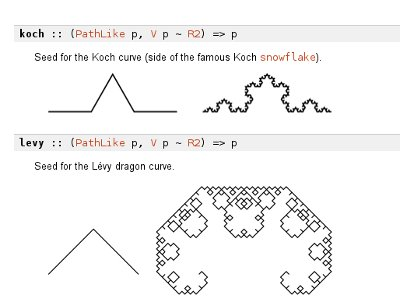
\includegraphics[width=0.4\textwidth]{html/diagrams-haddock.jpg}
% \end{center}
% %*endignore

There have been many improvements and changes to the core
diagrams libraries as well.  A 1.0 release is planned for on or around
November 20, to coincide with Brent's presentation at the New York
Haskell Users' Group.  Features slated for the 1.0 release
include:
\begin{itemize}
\item A nice API for drawing arrows between arbitrary points or diagrams.
\item Convenient integration with the \texttt{lens} package.
\item Path offsets and expansions: for example, the operation of
  ``stroking'' a path can now be internalized within diagrams,
  returning a closed path representing the outline of the stroke.
\item Performance improvements: across-the-board improvements of
  around 30\%, and more optimized SVG output.
\end{itemize}

%**<img width=350 src="./PythagoreanTree.png">
%*ignore
\begin{center}
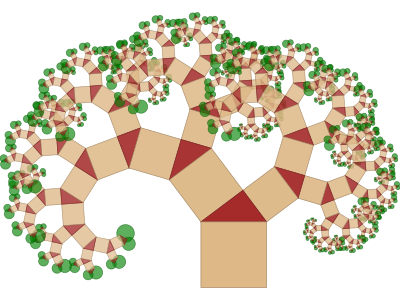
\includegraphics[width=0.235\textwidth]{html/PythagoreanTree.png}
\end{center}
%*endignore


%**<img width=350 src="./FibCalls.png">
%*ignore
\begin{center}
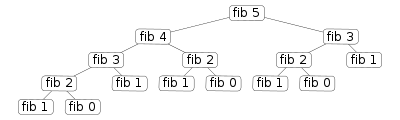
\includegraphics[width=0.33\textwidth]{html/FibCalls.png}
\end{center}
%*endignore

\subsubsection*{Contributing}

There is plenty of exciting work to be done; new contributors are
welcome!  Diagrams has developed an encouraging, responsive, and fun
developer community, and makes for a great opportunity to learn and
hack on some ``real-world'' Haskell code.  Because of its size,
generality, and enthusiastic embrace of advanced type system features,
diagrams can be intimidating to would-be users and contributors;
however, we are actively working on new documentation and resources to
help combat this.  For more information on ways to contribute and how
to get started, see the Contributing page on the diagrams wiki:
\url{http://haskell.org/haskellwiki/Diagrams/Contributing}, or come
hang out in the \texttt{\#diagrams} IRC channel on freenode.

%**<img width=400 src="./tree500.jpg">
%*ignore
\begin{center}
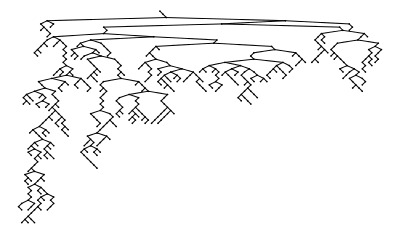
\includegraphics[width=0.4\textwidth]{html/tree500.jpg}
\end{center}
%*endignore

\FurtherReading
\begin{compactitem}
\item \url{http://projects.haskell.org/diagrams}
\item \url{http://projects.haskell.org/diagrams/gallery.html}
\item \url{http://haskell.org/haskellwiki/Diagrams}
\item \url{http://github.com/diagrams}
\item \url{https://byorgey.wordpress.com/2012/08/28/creating-documents-with-embedded-diagrams/}
\item \url{http://www.cis.upenn.edu/~byorgey/pub/monoid-pearl.pdf}
\item \url{http://www.youtube.com/watch?v=X-8NCkD2vOw}
\end{compactitem}
\end{hcarentry}
